\documentclass{article}
\usepackage{graphicx}
\usepackage{geometry}
\geometry{hmargin=2.5cm,vmargin=1.5cm}
\usepackage[utf8]{inputenc}
\usepackage{hyperref}

\begin{document}

\title{Un mini jeu de quête à-la-rogue}

\date{Hackthon du 29 janvier 2021}

\author{UE 12 informatique - apprentissage de la programmation - année
  2020-2021}

\maketitle

\begin{abstract}
l'idée est de réaliser un petit jeu similaire, dans son aspect
général, au célèbre jeu vidéo Rogue
\end{abstract}

\section{Introduction}

Rogue est un jeu de parcours de donjons qui se joue sur un simple
terminal.

Si vous ne le connaissez pas encore, parcourez la page Wikipédia ici
\url{https://en.wikipedia.org/wiki/Rogue\_(video\_game)} ou essayer le
jeu (pas trop longtemps) là
\url{https://archive.org/details/msdos\_Rogue\_1983}.

Vous savez enfin ce à quoi les élèves jouaient en 1983...

\vspace{.2cm}
\begin{center}
  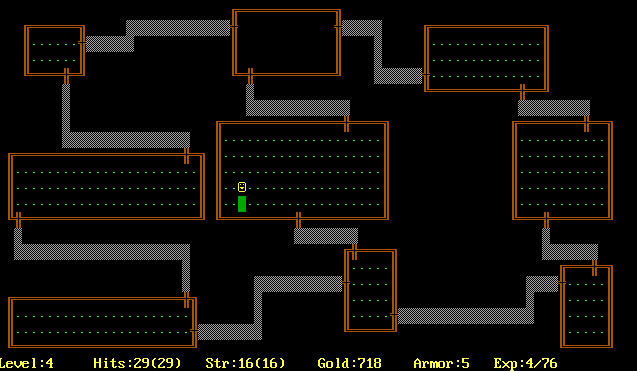
\includegraphics[width=3.0in]{Rogue_Screen_Shot_CAR.png}
  
  rogue - wikipedia
\end{center}

\section{Le jeu}

Le but de ce sujet est très simple~: vous devez vous inspirez de rogue
pour réaliser votre propre jeu de donjon.

\subsection{La forme graphique du jeu}

Votre jeu aura une interface graphique, pour les c++ basée sur un
terminal (\texttt{ncurses}), pour les Python basée sur
\texttt{pygame}, pour les java sur \texttt{awt} ou autre librairie
suggérée par votre professeur.

Mais surtout, pensez à faire les choses de \textbf{manière graduelle}
et pensez à commiter sous \texttt{git} à chaque fois que vous avez
quelque chose qui marchouille.

\vspace{.3cm}

Dans la suite de ce document, nous allons expliciter le jeu pour c++,
pour les autres langages vous adapterez la présentation à la librairie
choisie.

Animer un jeu par des caractères tapés et affichés dans un terminal,
vous permet de le prototyper rapidement. Ainsi, votre terrain du jeux
sera les lignes et les colonnes de votre terminal où la librairie
\texttt{ncurses} va vous permettre d'écrire des caractères (ou chaînes
de caractères) à la position désirée $(line, column)$.

Elle va vous permettre aussi de lire des caractères (ou plutôt des
événements clavier) pour contrôler le jeu (par exemple les flèches
pour déplacer le personnage).

\subsection{À quoi ressemblait le premier jeu Rogue}

Nous vous donnons ci-dessous très rapidement quelques idées sur la
manière (approximative) dont fonctionnait Rogue.

Vous êtes libres de vous en inspirer, ou pas du tout (faites alors
comme vous voulez) !

\vspace{.3cm}

Votre \textsl{personnage} (le caractère \texttt{'@'}) erre dans un
donjon à la recherche d'un Graal ou pour toute autre raison.

\vspace{.3cm}

Le donjon est constitué de \texttt{'|'} et de \texttt{'-'} pour les
murs, de \texttt{'.'} pour le sol, de '+' pour les portes, de
\texttt{'='} pour les escaliers, de \texttt{'\#'} pour les couloirs.

\begin{verbatim}
   --------    -------
   |.@....|  ##+.....|   #####
   |......|  # |.....|   #   #
   |......+### |.....+####   #
   |......|    |.....|       #
   |......| ###+.....|       #
   |......| #  ----+--   #####
   ----+--- #     #      #
       #    #     #    --+---
       #    #     #    |....|
       ############    |...=|
                       ------
\end{verbatim}
\begin{center}
  \textit{figure: '@' dans la première pièce d'un niveau de 3 pièces}
\end{center}

Pour les Python vous pouvez vous inspirer des techniques que vous avez
utilisées pour le snake.

Notons qu'il est plus intéressant pour le jeu que le donjon se
découvre petit à petit quand le personnage avance mais que dans un
premier temps, il peut être visible.
 
\vspace{.3cm}

Au cours de sa quête, votre personnage rencontre des ennemis (comme le
terrible chevalier noir \texttt{'B'}) qu'il doit combattre
vaillamment. L'issu du combat n'est jamais sûre, votre personnage
s'affaiblit quand il recoit des coups de son ennemi (ses points de vie
diminuent) il peut mourir (il n'a plus de points de vie), quand il en
sort vainqueur il s'améliore (sa force augmente, il peut aussi gagner
des points de vie).


\begin{verbatim}
   --------    -------
   |.@....|  K#+.....|   #####
   |......|  # |.....|   #   #
   |......+### |.....+####   #
   |......|    |.....|       #
   |......| ###+.....|       #
   |......| #  ----+--   #####
   ----+--- #     #      #
       #    #     #    --+---
       #    #     #    |....|
       ############    |...=|
                       ------
\end{verbatim}
\begin{center}
  \textit{figure: '@' ne voit pas encore 'K' caché dans couloir}
\end{center}

\vspace{.3cm}

Votre personnage va trouver des trésors et des objets durant sa quête.

De l'or \texttt{'*'} qu'il pourra utiliser pour soudoyer un gardien,
acheter des objets dans un magasin ou s'enrichir personnellement.

Des potions magiques \texttt{'j'} qu'il peut ramasser, placer dans son
sac pour les boire plus tard ou boire tout de suite au dépend de sa
vie (les potions peuvent l'affaiblir, lui apporter des pouvoirs
magiques, de la force...).

Des armes (poignards, dagues et épées \texttt{'!'}, arcs et flèches
\texttt{'('} qu'il peut ramasser, placer dans son sac et prendre en
main pour combattre des monstres.

Des armures ou casques \texttt{'\&'} pour se protége, des parchemins,
des anneaux \texttt{'o'} qui peuvent avoir des pouvoirs quand le
personnage les enfile.

De la nourriture parce que votre personnage ne doit pas mourir de faim
ni de soif.

Les objets peuvent être magiques alors attention aux mauvais sorts.

\begin{verbatim}
   --------    -------
   |.@....|  ##+...!.|   #####
   |......|  # |.&...|   #   #
   |......+### |.....+####   #
   |......|    |...o.|       #
   |..j...| ###+.....|       #
   |*.....| #  ----+--   #####
   ----+--- #     #      #
       #    #     #    --+---
       #    #     #    |....|
       ############    |...=|
                       ------
\end{verbatim}
\begin{center}
  \textit{figure: '@' avec une potion, de l'or, un poignard, un anneau, une armure.}
\end{center}

\vspace{.3cm}

Quand il marchera sur un objet, le jeu lui décrira l'objet et là soit
le jeu considère qu'il le prend automatiquement soit lui propose de le
prendre. Ainsi si \texttt{" votre personnage trouve 30 pièces d'or "},
celles-ci se rajoutent automatiquement à son porte-monnaie, si
\texttt{" votre personnage trouve une potion magique bleue ? pour la
  prendre faire) "}.

Pour les objets autre que l'or, son sac peut ne pas avoir une capacité
infinie. Votre personnage devra alors décider de jeter un objet pour
en garder un autre ou trouver sur son chemin un sac plus gros (y'en
a).

\vspace{.3cm}

Le personnages peut faire des actions par exemple comme se déplacer, monter
un escalier \texttt{'<'}, le descendre \texttt{'>'}, combattre, lire,
manger, boire, s'armer, enfiler une armure, mettre un casque, allumer
sa torche (des pièces peuvent être plongées dans l obscurité) ...
tout ce que vous voulez qu'il fasse.

\vspace{.3cm}

Et votre personnage peut enfin trouver le Graal...

\vspace{.3cm}

Le donjon a plusieurs niveaux (d'où les escaliers), une fois un niveau
exploré, votre personnage doit trouver le moyen d'accéder aux autres
niveaux.

Il peut y avoir des passages secrets, des trappes, certaines pièces
peuvent être dans l'obscurité... tout ce que vous imaginez.

\vspace{.3cm}

Et bien sûr, votre jeu peut être complètement différent.

\section{Parlons un peu d'organisation et de code...}

Vous êtes une équipe commencez par imaginer ensemble votre jeu et son
scénario: le personnage, les monstres, les trésors, la carte des
niveau, etc.

Déterminer les différents composants sur lesquels votre jeu sera
construit et comment ils s'interfacent.

Partagez vous les composants à réaliser. Vous devez garder à l'esprit
la vision globale de votre prototype de jeu.

Vous devrez avoir une manière de développer et tester chacun des
composants (un \textsl{build} par composant) et une manière de mettre
des composants ensemble (de les intégrer) et de tester le jeu (un
\textsl{build} général). Pour réunir les composants pensez à utiliser
git.

Et pensez aussi à commentez a-minima votre code pour que tout le
groupe puisse s'en servir facilement. Et à mettre des aides en lignes
pour en faciliter l'apprentissage. Genre le caractère '?'  affiche une
aide contextuelle.

Naturellement, pour chaque composant, prévoyez une gradation dans les
fonctionnalités à implémenter. Partez d'une version minimaliste et
complexifiez-la au fur et à mesure. Ne partez pas chacun bille en tête
à coder des tas de lignes de code sans jamais les compiler, les tester
et les intégrer !  vous ne convergerez pas facilement comme
cela. Pensez à avoir très rapidement un build d'un jeu minimaliste.

\section{Parlons rendu}

Nous sommes là pour répondre à vos questions et pour vous débloquer en
cas de problème.

En fin de journée nous allons organiser un rendu inspiré par la forme
du \textit{lightning-talk}: vous aurez un créneau de temps très court
(genre 3 minutes) pour faire une démo de votre jeu, ou de ce qui
fonctionne à ce moment là ... pensez-y quand vous créez vos
\textit{commits}.

\end{document}

